\chapter{Methods}

This section outlines the experimental procedures and processes carried out to conduct the research study. It includes datasets, the process of training and testing the model, and metrics used to evaluate the method's performance.

\section{Dataset}
The dataset provided by Siemens consists of images of Solder joints on a \gls{pcb}. It has a total of 6014 images, each of $512 \times $512 dimensions, divided into \gls{fc} and \gls{ng}. The \gls{fc} class contains images without defects, while the \gls{ng} class contains images with various defects. The images are of two types, one is a colored image, as shown in the middle of figure\ref{fig:dataset-FC}, and the other is a heat image, which is the red one in figure\ref{fig:dataset-FC}. This variation of images makes it suitable for evaluating various images for which a model can be used. The dataset is split into training and testing sets using an 80-20 split. A separate set of 160 images is also reserved for testing, finding accuracy, and visualizing classification and segmentation results.

\begin{figure}[ht!]
    \centering  
    \begin{minipage}{0.32\textwidth}
        \centering
        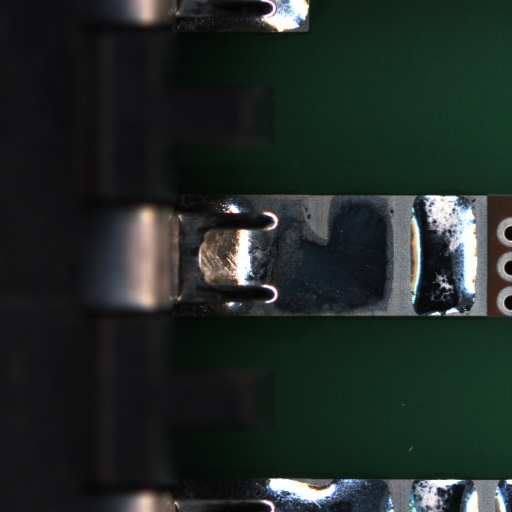
\includegraphics[width=\textwidth]{Images/Val_NG_BF2003043437_151_7_816_816_Color_origin.jpg} % Add your image file name here
        %\caption{An example of a defective piece of leather.}
    \end{minipage}
    \begin{minipage}{0.32\textwidth}
        \centering
        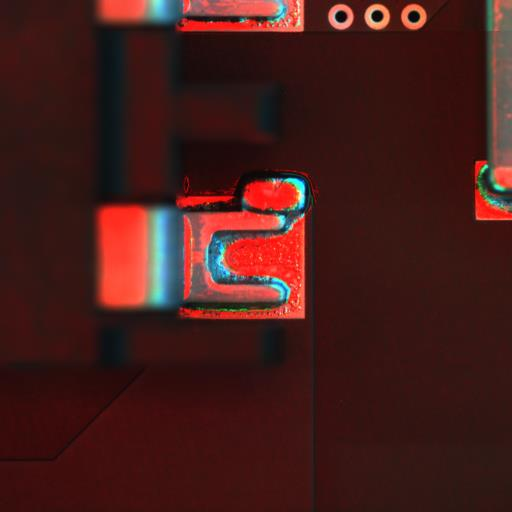
\includegraphics[width=\textwidth]{Images/Val_NG_BF2003033542_223_32_471_471_Multi_origin.jpg} % Add your image file name here
        %\caption{An example of a defective grid.}
    \end{minipage}\hfill
    \caption{Examples of defective solder joints in the dataset.}
    \label{fig:dataset-NG}
\end{figure}

\begin{figure}[ht!]
    \centering
    \begin{minipage}{0.32\textwidth}
        \centering
        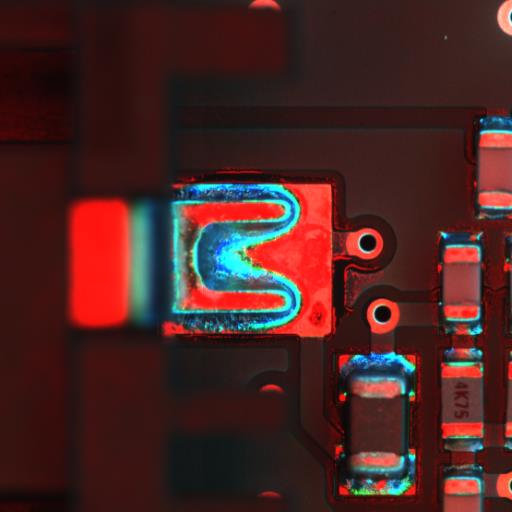
\includegraphics[width=\textwidth]{Images/Val_FC_heat_BF2003054784_4796_144_2042_2042_Multi.jpg} % Add your image file name here
        %\caption{An example of a defective tile.}
    \end{minipage}   
    \begin{minipage}{0.32\textwidth}
        \centering
        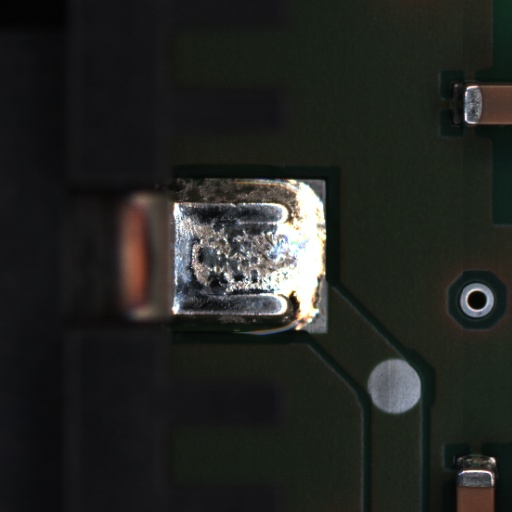
\includegraphics[width=\textwidth]{Images/train_FC_BF2003015014_1174_42_2038_2038_Color.jpg} % Add your image file name here
        %\caption{An example of a defective piece of leather.}
    \end{minipage}\hfill
    \caption{Examples of defect-free solder joints in the dataset.}
    \label{fig:dataset-FC}
\end{figure}

As can be seen in figure \ref{fig:dataset-NG} and figure \ref{fig:dataset-FC}, finding a defect without expertise can be challenging and time-consuming.

The table~\ref{tab:dataset-distribution} provides a detailed breakdown of the dataset distribution across subsets:

\begin{table}[ht!]
    \centering
    \begin{tabular}{|l|c|c|c|}
        \hline
        \textbf{Dataset} & \textbf{FC (No Defects)} & \textbf{NG (Defective)} & \textbf{Total} \\
        \hline
        Training & 2,971 & 1,712 & 4,683 \\
        \hline
        Testing & 743 & 428 & 1,171 \\
        \hline
        Custom Test & 80 & 80 & 160 \\
        \hline
    \end{tabular}
    \caption{Distribution of Images in the Dataset}
    \label{tab:dataset-distribution}
\end{table}

\section{Experiment}

Experiments were carried out using models mentioned in the [Theory section]. All the models belong to Anomaly detection and are part of a deep learning library which has a collection of state-of-the-art anomaly detection algorithms called Anomalib. There are multiple steps taken in this experiment and they will be explained below.

\subsection{Data Loading}

To load and preprocess our dataset, we use Anomalib dataloader by importing \textbf{Folder} from \textbf{Data} class, specifically designed for handling our custom dataset, allowing for efficient data management and preprocessing. We create a Folder datamodule and configure several parameters as described below.

\textbf{Name :} It is designated as the dataset configuration identifier, reflecting the specific dataset used for the experiment.

\textbf{Root Directory :} It points to the directory containing the organized dataset folders.

\textbf{Normal \& Abnormal Directories :} Models mostly require anomalous free images for training, which in our case is \gls{fc}, and anomalous images for testing(not used while training), which is \gls{ng}. So those are provided in these two fields.

\textbf{Normal Split Ratio :} The datamodule employs a 0.2 split ratio for validating normal images, which ensures a sufficient number of samples for model tuning and validation.

\textbf{Image Size :} All images are resized to $256 \times 256$ pixels during preprocessing, balancing the need for detailed feature representation with computational efficiency.

\textbf{Batch Size :} Both training and evaluation processes use different batch sizes for different models explained in [chapter 2] to optimize \gls{gpu} memory usage while maintaining effective gradient updates.

\textbf{Task Type :} There are two types of tasks available: classification and segmentation. For this thesis, for all the models, we have set the parameter to "CLASSIFICATION" and it directs the model to perform binary classification between the \gls{fc} and \gls{ng} categories.

\textbf{Number of Workers :} Based on the \gls{gpu} and the model being used, the number of workers varied between 0 to 8 for helping the computational resources to parallelize data loading.

Model loading is carried out by importing. Here, each model is configured with a specific backbone, which serves as a feature extraction component. 

\subsection{Model Training or Inferencing}
\label{subsec:Model Training}

The training takes place in two steps here: first is loading the model, and second is the training part, which is explained below.

\textbf{Model Loading :} Firstly, the model of our choice is imported. The models used in this thesis are explained in \ref{sec:unsupervised image processing}. Each model is initialized with a specific backbone, such as '\gls{resnet}18', '\gls{resnet}50', 'Wide\gls{resnet}50' etc. These backbones are critical for feature extraction. The selection of the backbone and the specific layers used for feature extraction are the key factors that influence the model's ability to detect anomalies.

\textbf{Model Training or Inferencing :} Once the model is loaded, the next steps involve training or inferencing using the \textbf{Engine} class from Anomalib. Depending on the model we need to either train the model or just perform inferencing(extracting the features). The engine is configured to manage the complete process, ensuring that the model is trained effectively and can accurately infer from the data provided.

The key components of training/inferencing configuration are:

\textbf{Thresholding :} A threshold value determines the anomalous label for the calculated anomaly scores. There are two types of thresholding methods available; one is '\textbf{ManualThreshold}' where we have to set our own threshold value; this is beneficial in situations where there is a lack of appropriate representative validation data\cite{9897283}. The second one we have used is '\textbf{F1AdaptiveThreshold}'. The algorithm optimizes the value of the threshold to determine the optimal f1\_score and saves the calculated value of the adaptive threshold.\cite{Anomalib2024}

\textbf{Task Type :} The task is usually set to '\textbf{CLASSIFICATION}', which directs the model to categorize images into predefined classes (ex., normal and anomalous). Depending on the requirements, the task can also be configured to '\textbf{SEGMENTATION}' to pinpoint where the defect is there in the image.

\textbf{Image Metrics :} The model's performance is evaluated by '\textbf{\gls{auroc}}' and '\textbf{F1Score}'. These are standard metrics used for assessing classification accuracy and balance between precision and recall. These metrics will be explained in section \ref{subsec:Evaluation Metrics}.

\textbf{Accelerator :} Depending on the available resources, the engine can run on a \textbf{'\gls{gpu}'}, \textbf{'\gls{cpu}'}, \textbf{'\gls{tpu}'}, \textbf{'\gls{ipu}'}, also there is an \textbf{'auto'} which chooses the appropriate resource automatically based on the availability.

\textbf{Devices :} This configuration allows us to provide the engine with the available number of devices(ex., \glspl{cpu}, \glspl{gpu}) to use during training and inference. The \textbf{'auto'} option sets the optimal devices automatically for the engine.

\textbf{Validation Frequency :} After every epoch \textbf{'check\_val\_every\_n\_epoch=1'}, this option validates the model, ensuring that the performance metrics are tracked throughout the training process.

\textbf{Max Epochs :} Depending on the model we are using, it can either required to be trained or do inferencing on. When the model performs inferencing at that time, the \textbf{'max\_epochs'} parameter is always set to \textbf{1}. Moreover, the models requiring training can be adjusted depending on the complexity of the model.%might need to add more info.

\textbf{Validation Check Interval :} The parameter \textbf{'val\_chedck\_interval'} sets when the validation checks are performed, in our case, it's set to \textbf{1.0}, meaning the validation checks are performed after every epoch.

After providing these training configurations to the engine class, we can call the \textbf{fit} function to start with the training or inferencing. Here, we provide the model and the datamodule components. Here, the \textbf{Normal} directory is used, which is the anomaly free images. After the training/inferencing is finished, the next step is to perform testing, which is explained in the section below.

\subsection{Testing}

After the training/inferencing is finished, we can move to the next critical step, i.e., to evaluate the model's performance. For this, the \textbf{test} function from the engine class is used, and similar to the fit function, we again need to pass the model and the datamodule components. Here, the \textbf{Abnormal} directory is used, which has the anomalous images. 

After the testing, its results are displayed, with two metrics mentioned in section \ref{subsec:Evaluation Metrics} \gls{auroc} and F1-Score.

\subsection{Model Exporting}
\label{subsec:Model Exporting}

Exporting a trained model is a very important task, as the model can then be deployed in real-world applications. This process involves converting the trained model into a format optimized for efficient inference on various hardware, like \glspl{cpu}, \glspl{gpu} etc. Thus, the model can be incorporated into production environments, operating at scale by processing new data and identifying anomalies in real time.

The Anomalib library lets us convert the models into formats like OpenVINO, ONNX, etc. We export our models into OpenVINO format. OpenVINO is an open-source software toolkit used to optimize and deploy \gls{dl} models. It minimizes resource requirements and effectively deploys on various platforms like the cloud. OpenVINO\textsuperscript{TM} enables inference on several hardware platforms, including \glspl{cpu}, \glspl{gpu}.\cite{openvino2024}

The export process is initialized by setting the desired export format via the \textbf{'ExportType'} variable. The trained model and the destination where the model should be exported are then passed to the \textbf{'Export'} function present in the engine class, which is responsible for the conversion. In the specified export location, three files are saved there:

\textbf{1. 'metadata.json'}, which stores the threshold value as mentioned in the section \ref{subsec:Model Training} based on which the classification can be done.

\textbf{2. 'model.bin'} is a binary file that contains the weights and biases of the model.

\textbf{3. 'model.xml'} this file stores the model's architecture. It contains the neural network structure, including layers, the connections between them, etc.

\section{Inference}
\label{subsec:Inference}

In the inference phase, the model is utilized to make predictions on new and unseen data. This section documents the approaches for achieving inference using a trained model, mainly focusing on two tasks: \textbf{'Image Classification'} and \textbf{'Image Segmentation'}. Both tasks are crucial in assessing the effectiveness of the model in detecting and localizing anomalies in solder joints on \glspl{pcb}.

Firstly, the trained model is loaded using the \textbf{'OpenVINOInferencer'} or \textbf{'TorchInferencer'} class, which can enable efficient inference on \glspl{cpu} or \glspl{gpu} respectively. Here, we will be using OpenVINOInferencer by providing the model and metadata paths of the trained model as explained in the section \ref{subsec:Model Exporting}. Once we are done creating the \textbf{'Inferencer'} object, we can move on to performing image classification and segmentation as described below.

\subsection{Image Classification}
\label{subsec:Image Classification}

Image Classification is an important task within \gls{cv} because it helps identify and recognize the object present in an image. It involves labeling input images based on their likelihood of being anomalous or not \cite{FANG2020100980}.

As mentioned in section \ref{subsec:Inference}, after creating the inference object then, we pass the input image to its \textbf{'predict'} function, which calculates the predicted label and the anomalous score. The predicted results are then visualized using \textbf{'ImageVisualizer'} class, which is configured for \textbf{CLASSIFICATION} mode, so it overlays the classification results on the input image, making it simpler to analyze the results.

\begin{figure}[ht!]
    \centering
    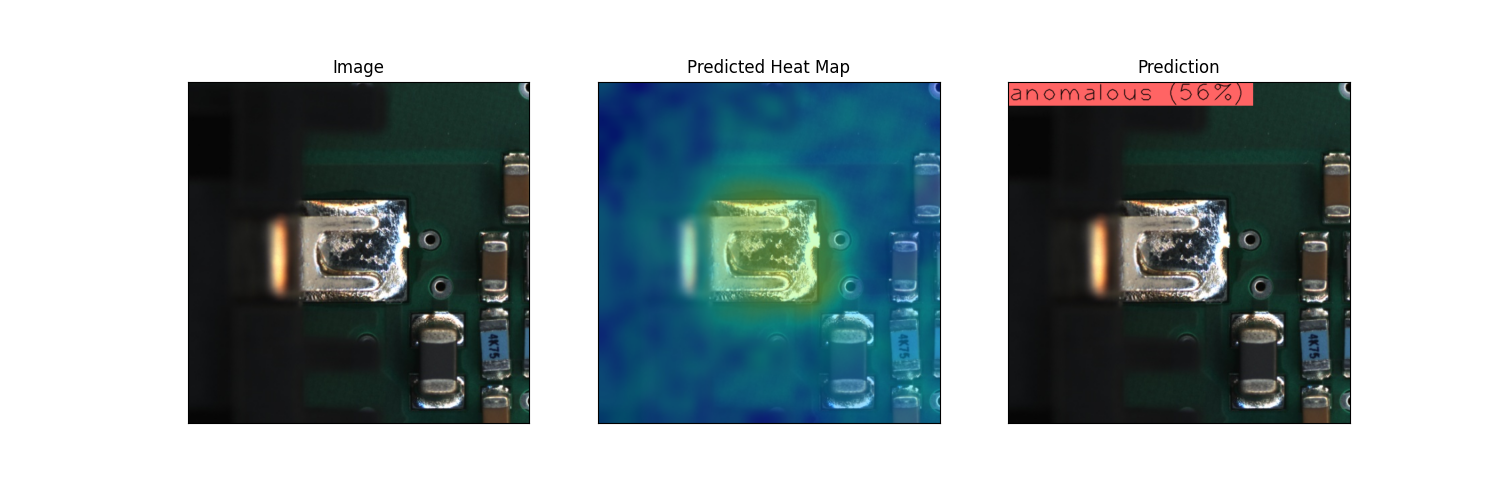
\includegraphics[width=1\linewidth]{Images/anomalous_image_classification.jpg}
    \caption{Image Classification on NG image}
    \label{fig:Image classification on NG image}
\end{figure}

Figure \ref{fig:Image classification on NG image} shows the result of image classification, where it gives three images as an output: one is the input image, the second one shows the predicted heat map, which shows where the possible anomaly and the third gives the prediction label and the score.

\subsection{Image Segmentation}
%\subsubsection{Metrics Calculation}

Image segmentation is a method of analyzing images at the pixel level. It involves utilizing multiple techniques to label each pixel as part of a particular class or instance\cite{IBM2024}. So, using image segmentation, we can point where the model has predicted the anomaly to be as shown in the figure \ref{fig:Image Segmentation on NG image}.

\begin{figure}[ht!]
    \centering
    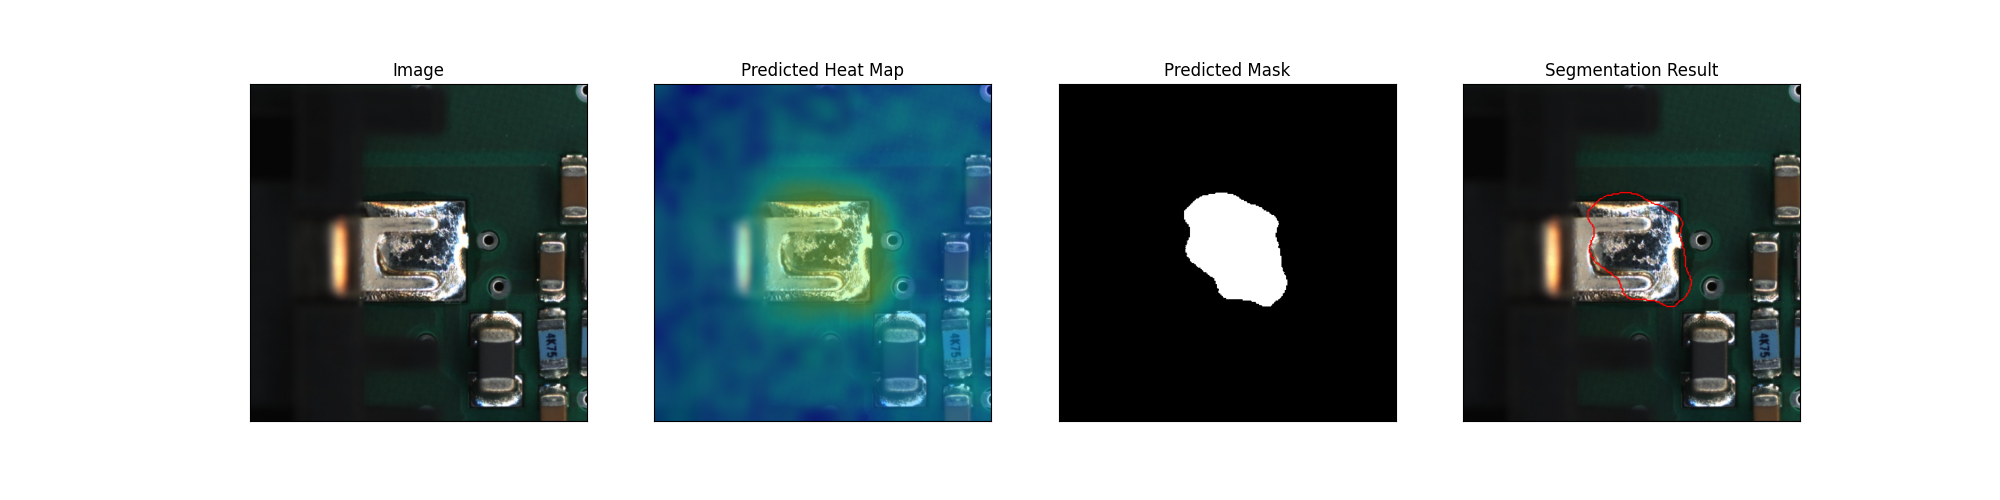
\includegraphics[width=1\linewidth]{Images/anomalous_image_segmentation.jpg}
    \caption{Image Segmentation on NG image}
    \label{fig:Image Segmentation on NG image}
\end{figure}

\section{Evaluation Metrics}
\label{subsec:Evaluation Metrics}

Evaluation metrics play a crucial role in determining how well the performance of a \gls{ml} model. These metrics aid in quantifying the model's ability to differentiate between anomalous and normal images, offering valuable insights into the model's effectiveness and areas for improvement. This section outlines the primary evaluation metrics utilized in this thesis: AUROC, Accuracy, Recall, Precision, F1-Score, and Confusion Matrix.

\subsection*{Area Under the Receiver-Operating Curve (AUROC)}
\label{subsec:AUROC}

The \gls{auroc} measures the ability of a classification model to differentiate across different classes. It has been particularly useful in measuring trade-offs of the \gls{tpr} (sensitivity) versus the \gls{fpr} (1-specificity) across different threshold settings. A higher \gls{auroc} value indicates better model performance, with a value of 1 representing a perfect model and a value of 0.5 indicating that the model that performs no better than random chance\cite{FAWCETT2006861}. This is extremely important for quality control applications because missing an anomaly can have severe consequences for a manufacturing process. %Write how its calculated in anomalib if possible

\subsection*{Accuracy}
\label{subsec:Accuracy}

Accuracy is the rate of correct predictions made by the model. It is often assessed using an unseen dataset that was never utilized throughout the learning process, like the custom test set mentioned in the table \ref{tab:dataset-distribution}.\cite{Kohavi1998}. It is expressed as: 

\begin{equation}
    \text{Accuracy} = \frac{\text{\gls{tp}} + \text{\gls{tn}}}{\text{\gls{tp}} + \text{\gls{tn}} + \text{\gls{fp}} + \text{\gls{fn}}} \quad \text{\cite{Walker2024}}
    \label{eq:accuracy}
\end{equation}

Where \gls{tp}, \gls{tn}, \gls{fp}, and \gls{fn} are True Positives, True Negatives, False Positives, and False Negatives, respectively. It gives an overall view of the performance of the model.

\subsection*{Recall}
\label{subsec:Recall}

Recall, also known as sensitivity, refers to the ratio of accurately predicted positive cases to the total number of actual positive cases \cite{powers2020evaluationprecisionrecallfmeasure}. It is expressed as:

\begin{equation}
    \text{Recall} = \frac{\text{\gls{tp}}}{\gls{tp} + \gls{fn}} \quad \text{\cite{powers2020evaluationprecisionrecallfmeasure}}
    \label{eq:recall}
\end{equation}

A higher Recall value means that the model is good at detecting most anomalies, but it does not consider the number of \gls{fp}.

\subsection*{Precision}
\label{subsec:Precision}

Precision, also known as confidence, refers to the proportion of accurately predicted positive cases that are actually correct \cite{powers2020evaluationprecisionrecallfmeasure}. It is expressed as:

\begin{equation}
    \text{Precision} = \frac{\text{\gls{tp}}}{\gls{tp} + \gls{fp}} \quad \text{\cite{powers2020evaluationprecisionrecallfmeasure}}
    \label{eq:precision}
\end{equation}

This metric is very important where the cost of false positives is high, as it indicates how well the model can prevent the incorrect labeling of normal cases as anomalies. 

\subsection*{F1-Score}
\label{subsec:F1-Score}

The F1-score is a metric that achieves a balance between precision and recall. The calculation involves taking the harmonic mean of precision and recall. The F1-score is a valuable metric for achieving a trade-off between high precision and recall. It effectively penalizes extreme negative values of either component \cite{Walker2024}. It is expressed as:

\begin{equation}
\text{F1-Score} = 2 \times \frac{\text{Precision} \times \text{Recall}}{\text{Precision} + \text{Recall}} \quad \text{\cite{Walker2024}}
\end{equation}

It makes this metric valuable since it evaluates a models capability to detect anomalies(Recall) and its precision in identifying true positives without an excessive number of false positives. 

\subsection*{Confusion Matrix}
\label{subsec:Confusion Matrix}

A confusion matrix simply shows the predicted and actual classifications made by the model \cite{Kohavi1998}. It is a table containing the \gls{tp}, \gls{tn}, \gls{fp}, and \gls{fn} values. Subsequently, a Confusion Matrix can help explain the errors a model makes so that improvements can be made specifically within the same area.

\begin{figure}[ht!]
    \centering
    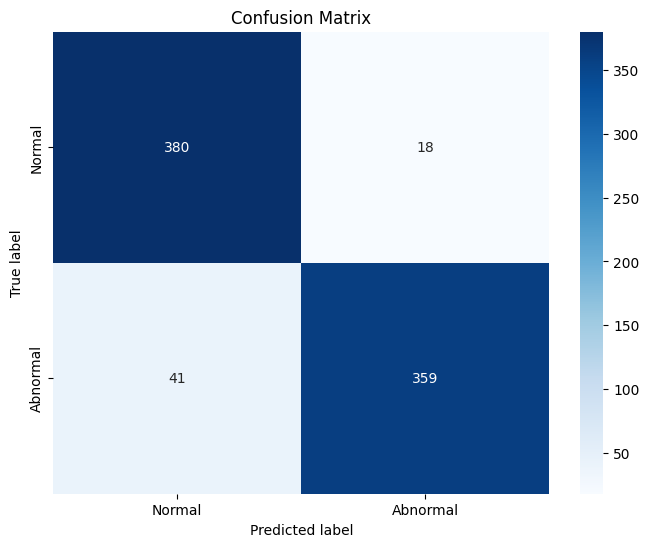
\includegraphics[width=1\linewidth]{Images/confusion matrix.png}
    \caption{Example of Confusion Matrix}
    \label{fig:confusion matrix}
\end{figure}

Figure \ref{fig:confusion matrix} shows a confusion matrix from one of our models. Here, the \gls{tp} is the top-left corner dark blue cell, \gls{tn} is the bottom-right dark blue cell, \gls{fp} is the bottom-left light blue cell, and \gls{fn} is the upper-right light blue cell.


